\chapter{Partikelrörelse i celler}

Partikelrörelse i cellers cytoplasma är något som länge fascinerat forskare inom området. En enkel modell som modellerar partikelrörelserna som klassisk brownsk rörelse kan inte förklara de observerade egenskaperna där en långsammare diffusion är ett av de mest tydliga exemplen. Andra modeller har tagits fram i avsikt att försöka förklara rörelsen men i dagsläget finns inte någon universell modell som kan beskriva rörelsen fullständigt. 

Detta kapitel presenterar inledningsvis tre möjliga förklaringsmodeller till partikelrörelsen:  Ornstein-Uhlenbeck-processen, CTRW och fBm som alla tre har kopplingar till klassisk brownsk rörelse. 

I detta arbete undersöks om given data över partikelrörelse i jästceller har egenskaper, bland annat MSD och asphericity, som kan beskrivas av dessa modeller. Både teoretiska beräkningar och simuleringar används för att göra jämförelsen. Den stora skillnaden mellan CTRW och fBm är att CTRW är en icke-stationär process medan fBm är stationär, något som används för att avgöra deras relevans som förklaringsmodeller. \todo{Är O-U stationär?}

Några av de viktigaste resultaten som presenteras i detta kapitel är att rörelsen verkar vara stationär och att ... \todo{Här kan man fylla i det man tycker är relevant}



\section{Alternativa modeller för partikelrörelse i vätskor}

Till en första approximation skulle alltså rörelsen för en partikel i en jästcells cytoplasma kunna beskrivas med klassisk brownsk rörelse. Partiklarna krockar där med mindre partiklar från omgivningen och rörelsen kan här beskrivas med en stokastisk gaussisk propagator~\cite{Einstein1905}
\begin{equation}
P(x,t)=\frac{1}{\sqrt{4\pi Dt}}e^{-\nicefrac{x^2}{4Dt}}
\end{equation} %Obs n=1 då endast en partikel följs
som utgörs av sannolikhetsfunktionen för partikelns förflyttning $x$ vid en given tid $t$, där konstanten $D$ är dess diffusionskonstant. Om partikeln betraktas som en sfär med radie $r$ nedsänkt i en vätska med viskositet $\eta$ och absolut temperatur $T$ kan $D$ approximeras till~\cite{Einstein1905}
\begin{equation}
D=\frac{RT}{N}\frac{1}{6\pi \eta r}
\end{equation}
där R är allmänna gaskonstanten och N antalet molekyler som ryms i 1 gram för omgivande fluiden.
\todo{Utveckla mer eller räcker det så här?}
%Man betraktar då cytoplasman som en homogen vätska. %Denna teori bygger dock på att man har termisk jämvikt och att partiklar rör sig i en enbart viskös vätska, två kriterier som inte uppfylls i cytoplasman bland annat på grund av mitokondriernas energiutvinning.

Experiment\cite{Midtveldt_etal2016} har dock visat att diffusionen av partiklar i celler är fundamentalt långsammare än förväntat från klassisk brownsk rörelse. Det finns ett par verktyg man kan använda för att undersöka detta. Ett av dem är MSD. Som visades i avsnitt~\ref{sec:brown} är MSD:n för brownsk rörelse proportionell mot förlupen tid. Speciellt kan \eqref{eq:MSD_brown} skrivas om till
\begin{equation}
\ev{x(t)^2} \propto t,
\end{equation}
där $x(0)=0$. Vad \cite{Midtveldt_etal2016} då har funnit i tidigare studier är att exponenten på $t$ är lägre än $1$, vilket tyder på att andra förklaringsmodeller kan behövas. %Två sådana kandidater är ''Continuous Time Random Walk'' (CTRW) och ''Fractional Brownian motion''.
\todo[inline]{Lägg in fler anledningar varför Brown inte funkar.}

%\subsubsection{Brownsk rörelse} \label{sec:Brownsk}
%\todo[inline]{Skriv ihop kort sammanfattning av det som står i stokastikavsnittet}
%\todo[]{Förklara varför anomal transport ens är intressant att studera.}


\subsection{Ornstein-Uhlenbeck-process}
En första utvidgning av modellen för brownsk rörelse fås genom att lägga till en återförande term som drar partikeln mot någon medelpunkt. Detta är en så kallad Ornstein-Uhlenbeck-process
\begin{equation}\label{eq:SDE_o-u}
\pd_t x = -\gamma ( x-\bar{x} ) + \pd_t W,
\end{equation}
där $\gamma$ är en tidsskala som styr hur hårt bunden partikeln är till medelpositionen $\bar{x}$, och $\pd_t W$ är den stokastiska drivningen av partikeln som uppfyller $\ev{\pd_t W}=0$ och $\ev{\pd_t W(t)\pd_t W(t')} = \sigma^2\delta(t-t')$. Detta är en inte helt orimlig modell eftersom en partikel i en cell rimligtvis inte kan vandra hur långt som helst. Typiskt kommer en partikel att tränga ihop cytoplasmans beståndsdelar i den riktning som den rör sig åt, vilket leder till en återförande kraft.

Med hjälp av \eqref{eq:SDE_o-u} och metoderna från avsnitt~\ref{sec:brown} kan modellens kovarians och MSD härledas. Kovariansen i gränsen mot ett stationärtillstånd ($\gamma t\gg 1$) blir då
\begin{equation}\label{eq:COV_o-u}
\ev{x(t)x(t+\Delta{t})} \approx \frac{\sigma^2}{2\gamma} \ee^{-\gamma\Delta{t}},
\end{equation}
där $\bar{x}$ har satts till 0. Vidare kan också MSD beräknas till:
\begin{equation}\label{eq:MSD_o-u}
\ev{x(t)^2} 
\approx \frac{\sigma^2}{2\gamma} \left( 1-\ee^{-2\gamma t} \right),
%\approx \frac{\sigma^2}{2\gamma}t\qcomma \text{för } \gamma t\ll1
\end{equation}
med $\bar{x}=0$. Notera att både \eqref{eq:COV_o-u} och \eqref{eq:MSD_o-u} ger att variansen, då $\gamma t\gg 1$, blir konstant lika med~$\nicefrac{\sigma^2}{2\gamma}$ eftersom $\ev{x(t)}=\bar{x}=0$.

%Notera likheten här till den styrande SDE:n för brownsk rörelse.

%\todo[inline]{Kommer mera så småningom...}
  
\subsection{Continuous Time Random Walk (CTRW)}
En möjlig förklaringsmodell för anomal transport i celler utgörs av CTRW (Continuous-Time Random Walk)~\cite{Hofling&Franosch2013}. Här beskrivs rörelsemönstret av att partiklarna under majoriteten av tiden sitter bundna till olika nätliknande strukturer för att sedan plötsligt ta sig vidare till en ny position efter en viss väntetid. Positionsändringen och väntetiden beskrivs av två oberoende stokastiska variabler. 
MSD för denna typ av rörelse blir\cite{Barkai_CTRW}
\begin{equation}\label{eq:CTRW_MSD}
    \ev{x^2(t)} \approx \frac{\ev{\Delta x^2}}{A \Gamma(1+\alpha)}t^{\alpha} + \frac{2\ev{\Delta x}^2}{\Gamma(1+2\alpha)A^2} t^{2\alpha}, 
\end{equation}
där $A$ är en konstant som dyker upp i fördelningsfunktionen för väntetiderna, $\Gamma$ är gammafunktionen, $\alpha$ en konstant som uppfyller $0<\alpha<1$ och $\Delta x$ steget mellan två positioner. Om $\ev{\Delta x}=0 $ försvinner andra termen och rörelsens MSD blir proportionell mot $t^\alpha$. Eftersom $\alpha < 1$ blir MSD:n inte linjär i tiden, utan ändringstakten kommer att avta med tiden och rörelsen skiljer sig från den klassiska brownska rörelsen.
Denna anomala transport uppstår då medelväntetiden mellan två hopp blir oändlig så att centrala gränsvärdessatsen därmed ej uppfylls. Summan av de stokastiska variablerna går således ej mot att bli normalfördelad, något som är grundläggande i teorin kring brownsk rörelse. 

Teorin har visat sig kunna beskriva vissa aspekter av partikelrörelse i nät av F-aktin filament\cite{Barkai_CTRW}. Om partikelns radie var av samma storleksordning som genomsnittliga maskstorleken bands partiklarna tillfälligt i nätet, bortsett från termiska fluktuationer, för att sedan ta sig igenom en maska och fastna i ett nytt hålrum i nätet. MSD:n för dessa partiklar uppfyllde ett $t^{\alpha}$ beroende som i \eqref{eq:CTRW_MSD}. Partiklar med radie av mindre storleksordning än maskstorleken hade ett rörelsemönster mer likt brownsk rörelse medan de större partiklarna fastnade i nätet utan att kunna ta sig loss.
%Om en liknande nätstruktur kan uppstå i jästceller kan man alltså förvänta sig olika resultat vad gäller rörelsen för partiklar av olika storlek.

%Lästips:
%https://faculty.biu.ac.il/~barkaie/chapter4.pdf
%https://faculty.biu.ac.il/~barkaie/jstatBarkaiSokolov.pdf
%https://faculty.biu.ac.il/~barkaie/Pathways.pdf


\subsection{Fractional Brownian Motion (fBm)}

En annan modell som kan undersökas är fractional Brownian motion~\cite{Mandelbrot_fBm1968} som bygger på superpositioner av brownska processer med brus som uppvisar en beständig korrelation i tiden. 

Ett sätt att representera fBm är att utgå från en vanlig brownsk rörelse $B(t)$ och vikta tidigare steg i rörelsen med $((t-s)^{H-\nicefrac{1}{2}})$ så att fBm:n blir ett rörligt medelvärde av dB(t) enligt \cite{Mandelbrot_fBm1968}
\begin{equation}
    B_H(t,\omega)=\frac{1}{\Gamma(H+\nicefrac{1}{2})} \int_{\infty}^0 [(t-s)^{H-\nicefrac{1}{2}}-(-s)^{H-\nicefrac{1}{2}}]dB(s,\omega) + \int_0^t [(t-s)^{H-\nicefrac{1}{2}} dB(s,\omega)
\end{equation}
för $t>0$ utgående från startposition i 0 där $\omega$ representerar mängden av alla möjliga värden för den stokastiska funktionen och $\Gamma$ är gamma-funktionen. Hur denna typ av integral med stokastisk integrationsvariabel kan utföras förklaras i avsnitt \ref{sec:Stok_int}.
%Denna representation är dock inte unik \cite{Dieker_fBm}.

Mätningar på slumpfenomen har visat på starkt beroende även mellan brett spridda stickprov~\cite{Mandelbrot_fBm1968} något som inte kan förklaras med den brownska rörelsens exponentiellt avtagande korrelation \todo{Eller är det de okorrelerade stegen man avser här?}i ekvation \eqref{eq:Brown_korr}. Detta motiverar införandet av denna modell som kandidat för att beskriva   diffusion i celler. Modellen förutsäger också en minskad diffusionstakt jämfört med vanlig brownsk rörelse, något som observerats i verkliga celler ~\cite{Hofling&Franosch2013}.

En normaliserad fBm $B_H(t)$ kan karakteriseras helt från följande egenskaper\cite{Dieker_fBm}: $B_H(t)$ har stationära ökningar, gaussisk fördelning för $t>0$ och $B_H(0)=0$ samt att
\begin{align}
    \ev{B_H(t)}&=0 \\
    \ev{B^2_H(t)}&=t^{2H}
\end{align}
för $t\geq 0$ där Hurst parametern $H$ uppfyller $0< H <1$. För $H=\nicefrac{1}{2}$ återfås vanlig brownsk rörelse. Stationära ökningar medför att ($0<
t_1\leq t_2$)
\begin{equation}
    \ev{(B_H(t_1)-B_H(t_2))^2} = (t_1-t_2)^{2H},
\end{equation}
eller ekvivalent
\begin{equation}
    \ev{B_H(t_1)^2}+\ev{B_H(t_2)^2}-2\ev{B_H(t_1)B_H(t_2)} = (t_1-t_2)^{2H}.
\end{equation}
Kovariansen för fBm är således
\begin{equation}
\ev{B_H(t_1)B_H(t_2)}
= \frac{1}{2} \left(t_1^{2H}+t_2^{2H}-(t_2-t_1)^{2H}\right),
\end{equation}
vilket ger att för $H<\nicefrac{1}{2}$ fås positiv korrelation för två positioner i rörelsen och för  $H>\nicefrac{1}{2}$ fås negativ korrelation. Den negativa korrelationen ger brusigt utseende åt plotten över rörelsen då rörelsen ofta byter riktning medan den positiva korrelationen ger kurvan ett mer slätt utseende som tenderar att dra iväg i en bestämd riktning. Man kan även visa att fBm är den enda gaussiska process som uppträder självliknande \todo{Källa}[], det vill säga att $B_H(at)$ och $a^H B_H(t)$ har samma ändligtdimensionella fördelning.

Stegen mellan varje positionsändring $\Delta{B_H}_k=B_H(k+1)-B_H(k)$ är standardnormalfördelad för varje $k$ men tillskillnad från ren brownsk rörelse är stegen i allmänhet inte oberoende. Ovan utpekades dessa ökningars stationära egenskap som en av de karakteristiska dragen för fBm. Att ökningarna är stationära innebär att de saknar explicit tidsberoende, de beror bara på tidsintervallets storlek.

\todo[inline]{Mer om fysikalisk tolkning och vad den används till idag}
    
%Förväntad spektral densitet finns även i källan


%\section{Metod för dataundersökning} \todo[inline]{Inga tomma rubriker!}


\section{Intensitets- och storleksberoende}

%Om värdena skiljer sig åt väsentligt för små och stora partiklar -> CTRW mer trolig. 

\subsection{Resultat}

\begin{figure}\centering
\subfigure[][]{% GNUPLOT: LaTeX picture with Postscript
\begingroup
  \makeatletter
  \providecommand\color[2][]{%
    \GenericError{(gnuplot) \space\space\space\@spaces}{%
      Package color not loaded in conjunction with
      terminal option `colourtext'%
    }{See the gnuplot documentation for explanation.%
    }{Either use 'blacktext' in gnuplot or load the package
      color.sty in LaTeX.}%
    \renewcommand\color[2][]{}%
  }%
  \providecommand\includegraphics[2][]{%
    \GenericError{(gnuplot) \space\space\space\@spaces}{%
      Package graphicx or graphics not loaded%
    }{See the gnuplot documentation for explanation.%
    }{The gnuplot epslatex terminal needs graphicx.sty or graphics.sty.}%
    \renewcommand\includegraphics[2][]{}%
  }%
  \providecommand\rotatebox[2]{#2}%
  \@ifundefined{ifGPcolor}{%
    \newif\ifGPcolor
    \GPcolortrue
  }{}%
  \@ifundefined{ifGPblacktext}{%
    \newif\ifGPblacktext
    \GPblacktexttrue
  }{}%
  % define a \g@addto@macro without @ in the name:
  \let\gplgaddtomacro\g@addto@macro
  % define empty templates for all commands taking text:
  \gdef\gplbacktext{}%
  \gdef\gplfronttext{}%
  \makeatother
  \ifGPblacktext
    % no textcolor at all
    \def\colorrgb#1{}%
    \def\colorgray#1{}%
  \else
    % gray or color?
    \ifGPcolor
      \def\colorrgb#1{\color[rgb]{#1}}%
      \def\colorgray#1{\color[gray]{#1}}%
      \expandafter\def\csname LTw\endcsname{\color{white}}%
      \expandafter\def\csname LTb\endcsname{\color{black}}%
      \expandafter\def\csname LTa\endcsname{\color{black}}%
      \expandafter\def\csname LT0\endcsname{\color[rgb]{1,0,0}}%
      \expandafter\def\csname LT1\endcsname{\color[rgb]{0,1,0}}%
      \expandafter\def\csname LT2\endcsname{\color[rgb]{0,0,1}}%
      \expandafter\def\csname LT3\endcsname{\color[rgb]{1,0,1}}%
      \expandafter\def\csname LT4\endcsname{\color[rgb]{0,1,1}}%
      \expandafter\def\csname LT5\endcsname{\color[rgb]{1,1,0}}%
      \expandafter\def\csname LT6\endcsname{\color[rgb]{0,0,0}}%
      \expandafter\def\csname LT7\endcsname{\color[rgb]{1,0.3,0}}%
      \expandafter\def\csname LT8\endcsname{\color[rgb]{0.5,0.5,0.5}}%
    \else
      % gray
      \def\colorrgb#1{\color{black}}%
      \def\colorgray#1{\color[gray]{#1}}%
      \expandafter\def\csname LTw\endcsname{\color{white}}%
      \expandafter\def\csname LTb\endcsname{\color{black}}%
      \expandafter\def\csname LTa\endcsname{\color{black}}%
      \expandafter\def\csname LT0\endcsname{\color{black}}%
      \expandafter\def\csname LT1\endcsname{\color{black}}%
      \expandafter\def\csname LT2\endcsname{\color{black}}%
      \expandafter\def\csname LT3\endcsname{\color{black}}%
      \expandafter\def\csname LT4\endcsname{\color{black}}%
      \expandafter\def\csname LT5\endcsname{\color{black}}%
      \expandafter\def\csname LT6\endcsname{\color{black}}%
      \expandafter\def\csname LT7\endcsname{\color{black}}%
      \expandafter\def\csname LT8\endcsname{\color{black}}%
    \fi
  \fi
  \setlength{\unitlength}{0.0500bp}%
  \begin{picture}(4080.00,3968.00)%
    \gplgaddtomacro\gplbacktext{%
      \csname LTb\endcsname%
      \put(860,952){\makebox(0,0)[r]{\strut{}$10^{-9}$}}%
      \csname LTb\endcsname%
      \put(860,1990){\makebox(0,0)[r]{\strut{}$10^{-8}$}}%
      \csname LTb\endcsname%
      \put(860,3027){\makebox(0,0)[r]{\strut{}$10^{-7}$}}%
      \csname LTb\endcsname%
      \put(980,440){\makebox(0,0){\strut{} 0,1}}%
      \csname LTb\endcsname%
      \put(2122,440){\makebox(0,0){\strut{} 1}}%
      \csname LTb\endcsname%
      \put(3264,440){\makebox(0,0){\strut{} 10}}%
      \put(160,1833){\rotatebox{-270}{\makebox(0,0){\strut{}$\sigma_r$ /[m]}}}%
      \put(2349,140){\makebox(0,0){\strut{}$I$ /[godt. enhet]}}%
    }%
    \gplgaddtomacro\gplfronttext{%
      \csname LTb\endcsname%
      \put(3038,3755){\makebox(0,0)[r]{\strut{}\footnotesize Dvala}}%
      \csname LTb\endcsname%
      \put(3038,3555){\makebox(0,0)[r]{\strut{}\footnotesize Brusnivå}}%
      \csname LTb\endcsname%
      \put(3038,3355){\makebox(0,0)[r]{\strut{}\footnotesize Anpassning $\propto I^{-0,41}$}}%
    }%
    \gplbacktext
    \put(0,0){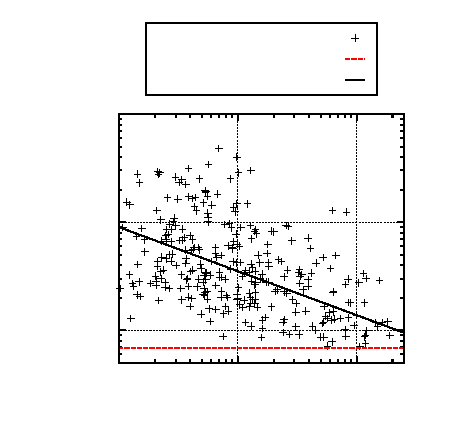
\includegraphics{std_ed}}%
    \gplfronttext
  \end{picture}%
\endgroup
}
\subfigure[][]{% GNUPLOT: LaTeX picture with Postscript
\begingroup
  \makeatletter
  \providecommand\color[2][]{%
    \GenericError{(gnuplot) \space\space\space\@spaces}{%
      Package color not loaded in conjunction with
      terminal option `colourtext'%
    }{See the gnuplot documentation for explanation.%
    }{Either use 'blacktext' in gnuplot or load the package
      color.sty in LaTeX.}%
    \renewcommand\color[2][]{}%
  }%
  \providecommand\includegraphics[2][]{%
    \GenericError{(gnuplot) \space\space\space\@spaces}{%
      Package graphicx or graphics not loaded%
    }{See the gnuplot documentation for explanation.%
    }{The gnuplot epslatex terminal needs graphicx.sty or graphics.sty.}%
    \renewcommand\includegraphics[2][]{}%
  }%
  \providecommand\rotatebox[2]{#2}%
  \@ifundefined{ifGPcolor}{%
    \newif\ifGPcolor
    \GPcolortrue
  }{}%
  \@ifundefined{ifGPblacktext}{%
    \newif\ifGPblacktext
    \GPblacktexttrue
  }{}%
  % define a \g@addto@macro without @ in the name:
  \let\gplgaddtomacro\g@addto@macro
  % define empty templates for all commands taking text:
  \gdef\gplbacktext{}%
  \gdef\gplfronttext{}%
  \makeatother
  \ifGPblacktext
    % no textcolor at all
    \def\colorrgb#1{}%
    \def\colorgray#1{}%
  \else
    % gray or color?
    \ifGPcolor
      \def\colorrgb#1{\color[rgb]{#1}}%
      \def\colorgray#1{\color[gray]{#1}}%
      \expandafter\def\csname LTw\endcsname{\color{white}}%
      \expandafter\def\csname LTb\endcsname{\color{black}}%
      \expandafter\def\csname LTa\endcsname{\color{black}}%
      \expandafter\def\csname LT0\endcsname{\color[rgb]{1,0,0}}%
      \expandafter\def\csname LT1\endcsname{\color[rgb]{0,1,0}}%
      \expandafter\def\csname LT2\endcsname{\color[rgb]{0,0,1}}%
      \expandafter\def\csname LT3\endcsname{\color[rgb]{1,0,1}}%
      \expandafter\def\csname LT4\endcsname{\color[rgb]{0,1,1}}%
      \expandafter\def\csname LT5\endcsname{\color[rgb]{1,1,0}}%
      \expandafter\def\csname LT6\endcsname{\color[rgb]{0,0,0}}%
      \expandafter\def\csname LT7\endcsname{\color[rgb]{1,0.3,0}}%
      \expandafter\def\csname LT8\endcsname{\color[rgb]{0.5,0.5,0.5}}%
    \else
      % gray
      \def\colorrgb#1{\color{black}}%
      \def\colorgray#1{\color[gray]{#1}}%
      \expandafter\def\csname LTw\endcsname{\color{white}}%
      \expandafter\def\csname LTb\endcsname{\color{black}}%
      \expandafter\def\csname LTa\endcsname{\color{black}}%
      \expandafter\def\csname LT0\endcsname{\color{black}}%
      \expandafter\def\csname LT1\endcsname{\color{black}}%
      \expandafter\def\csname LT2\endcsname{\color{black}}%
      \expandafter\def\csname LT3\endcsname{\color{black}}%
      \expandafter\def\csname LT4\endcsname{\color{black}}%
      \expandafter\def\csname LT5\endcsname{\color{black}}%
      \expandafter\def\csname LT6\endcsname{\color{black}}%
      \expandafter\def\csname LT7\endcsname{\color{black}}%
      \expandafter\def\csname LT8\endcsname{\color{black}}%
    \fi
  \fi
  \setlength{\unitlength}{0.0500bp}%
  \begin{picture}(3968.00,3400.00)%
    \gplgaddtomacro\gplbacktext{%
      \csname LTb\endcsname%
      \put(860,1058){\makebox(0,0)[r]{\strut{}$10^{-9}$}}%
      \csname LTb\endcsname%
      \put(860,2109){\makebox(0,0)[r]{\strut{}$10^{-8}$}}%
      \csname LTb\endcsname%
      \put(860,3159){\makebox(0,0)[r]{\strut{}$10^{-7}$}}%
      \csname LTb\endcsname%
      \put(980,440){\makebox(0,0){\strut{} 0}}%
      \csname LTb\endcsname%
      \put(1505,440){\makebox(0,0){\strut{} 5}}%
      \csname LTb\endcsname%
      \put(2031,440){\makebox(0,0){\strut{} 10}}%
      \csname LTb\endcsname%
      \put(2556,440){\makebox(0,0){\strut{} 15}}%
      \csname LTb\endcsname%
      \put(3082,440){\makebox(0,0){\strut{} 20}}%
      \csname LTb\endcsname%
      \put(3607,440){\makebox(0,0){\strut{} 25}}%
      \put(160,1899){\rotatebox{-270}{\makebox(0,0){\strut{}Medelstegläng /[m]}}}%
      \put(2293,140){\makebox(0,0){\strut{}Intensitet /[godt. enhet]}}%
    }%
    \gplgaddtomacro\gplfronttext{%
      \csname LTb\endcsname%
      \put(3064,2946){\makebox(0,0)[r]{\strut{}\footnotesize Energydepleted}}%
      \csname LTb\endcsname%
      \put(3064,2746){\makebox(0,0)[r]{\strut{}\footnotesize Brusnivå}}%
    }%
    \gplbacktext
    \put(0,0){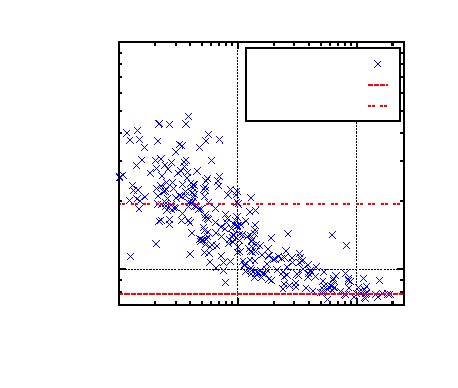
\includegraphics{medelsteg_ed}}%
    \gplfronttext
  \end{picture}%
\endgroup
}
\subfigure[][]{% GNUPLOT: LaTeX picture with Postscript
\begingroup
  \makeatletter
  \providecommand\color[2][]{%
    \GenericError{(gnuplot) \space\space\space\@spaces}{%
      Package color not loaded in conjunction with
      terminal option `colourtext'%
    }{See the gnuplot documentation for explanation.%
    }{Either use 'blacktext' in gnuplot or load the package
      color.sty in LaTeX.}%
    \renewcommand\color[2][]{}%
  }%
  \providecommand\includegraphics[2][]{%
    \GenericError{(gnuplot) \space\space\space\@spaces}{%
      Package graphicx or graphics not loaded%
    }{See the gnuplot documentation for explanation.%
    }{The gnuplot epslatex terminal needs graphicx.sty or graphics.sty.}%
    \renewcommand\includegraphics[2][]{}%
  }%
  \providecommand\rotatebox[2]{#2}%
  \@ifundefined{ifGPcolor}{%
    \newif\ifGPcolor
    \GPcolortrue
  }{}%
  \@ifundefined{ifGPblacktext}{%
    \newif\ifGPblacktext
    \GPblacktexttrue
  }{}%
  % define a \g@addto@macro without @ in the name:
  \let\gplgaddtomacro\g@addto@macro
  % define empty templates for all commands taking text:
  \gdef\gplbacktext{}%
  \gdef\gplfronttext{}%
  \makeatother
  \ifGPblacktext
    % no textcolor at all
    \def\colorrgb#1{}%
    \def\colorgray#1{}%
  \else
    % gray or color?
    \ifGPcolor
      \def\colorrgb#1{\color[rgb]{#1}}%
      \def\colorgray#1{\color[gray]{#1}}%
      \expandafter\def\csname LTw\endcsname{\color{white}}%
      \expandafter\def\csname LTb\endcsname{\color{black}}%
      \expandafter\def\csname LTa\endcsname{\color{black}}%
      \expandafter\def\csname LT0\endcsname{\color[rgb]{1,0,0}}%
      \expandafter\def\csname LT1\endcsname{\color[rgb]{0,1,0}}%
      \expandafter\def\csname LT2\endcsname{\color[rgb]{0,0,1}}%
      \expandafter\def\csname LT3\endcsname{\color[rgb]{1,0,1}}%
      \expandafter\def\csname LT4\endcsname{\color[rgb]{0,1,1}}%
      \expandafter\def\csname LT5\endcsname{\color[rgb]{1,1,0}}%
      \expandafter\def\csname LT6\endcsname{\color[rgb]{0,0,0}}%
      \expandafter\def\csname LT7\endcsname{\color[rgb]{1,0.3,0}}%
      \expandafter\def\csname LT8\endcsname{\color[rgb]{0.5,0.5,0.5}}%
    \else
      % gray
      \def\colorrgb#1{\color{black}}%
      \def\colorgray#1{\color[gray]{#1}}%
      \expandafter\def\csname LTw\endcsname{\color{white}}%
      \expandafter\def\csname LTb\endcsname{\color{black}}%
      \expandafter\def\csname LTa\endcsname{\color{black}}%
      \expandafter\def\csname LT0\endcsname{\color{black}}%
      \expandafter\def\csname LT1\endcsname{\color{black}}%
      \expandafter\def\csname LT2\endcsname{\color{black}}%
      \expandafter\def\csname LT3\endcsname{\color{black}}%
      \expandafter\def\csname LT4\endcsname{\color{black}}%
      \expandafter\def\csname LT5\endcsname{\color{black}}%
      \expandafter\def\csname LT6\endcsname{\color{black}}%
      \expandafter\def\csname LT7\endcsname{\color{black}}%
      \expandafter\def\csname LT8\endcsname{\color{black}}%
    \fi
  \fi
  \setlength{\unitlength}{0.0500bp}%
  \begin{picture}(3968.00,3400.00)%
    \gplgaddtomacro\gplbacktext{%
      \csname LTb\endcsname%
      \put(860,1058){\makebox(0,0)[r]{\strut{}$10^{-9}$}}%
      \csname LTb\endcsname%
      \put(860,2109){\makebox(0,0)[r]{\strut{}$10^{-8}$}}%
      \csname LTb\endcsname%
      \put(860,3159){\makebox(0,0)[r]{\strut{}$10^{-7}$}}%
      \csname LTb\endcsname%
      \put(980,440){\makebox(0,0){\strut{} 0}}%
      \csname LTb\endcsname%
      \put(1505,440){\makebox(0,0){\strut{} 5}}%
      \csname LTb\endcsname%
      \put(2031,440){\makebox(0,0){\strut{} 10}}%
      \csname LTb\endcsname%
      \put(2556,440){\makebox(0,0){\strut{} 15}}%
      \csname LTb\endcsname%
      \put(3082,440){\makebox(0,0){\strut{} 20}}%
      \csname LTb\endcsname%
      \put(3607,440){\makebox(0,0){\strut{} 25}}%
      \put(160,1899){\rotatebox{-270}{\makebox(0,0){\strut{}Standardavvikelse /[m]}}}%
      \put(2293,140){\makebox(0,0){\strut{}Intensitet /[godt. enhet]}}%
    }%
    \gplgaddtomacro\gplfronttext{%
      \csname LTb\endcsname%
      \put(3064,2946){\makebox(0,0)[r]{\strut{}\footnotesize Logphase}}%
      \csname LTb\endcsname%
      \put(3064,2746){\makebox(0,0)[r]{\strut{}\footnotesize Brusnivå}}%
    }%
    \gplbacktext
    \put(0,0){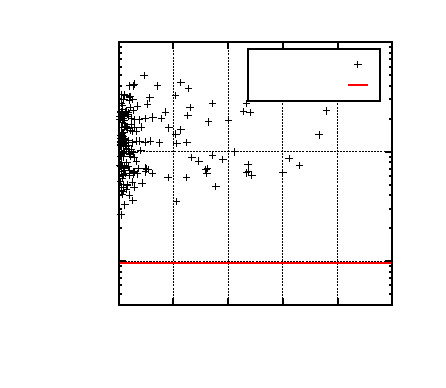
\includegraphics{std_lp}}%
    \gplfronttext
  \end{picture}%
\endgroup
}
\subfigure[][]{% GNUPLOT: LaTeX picture with Postscript
\begingroup
  \makeatletter
  \providecommand\color[2][]{%
    \GenericError{(gnuplot) \space\space\space\@spaces}{%
      Package color not loaded in conjunction with
      terminal option `colourtext'%
    }{See the gnuplot documentation for explanation.%
    }{Either use 'blacktext' in gnuplot or load the package
      color.sty in LaTeX.}%
    \renewcommand\color[2][]{}%
  }%
  \providecommand\includegraphics[2][]{%
    \GenericError{(gnuplot) \space\space\space\@spaces}{%
      Package graphicx or graphics not loaded%
    }{See the gnuplot documentation for explanation.%
    }{The gnuplot epslatex terminal needs graphicx.sty or graphics.sty.}%
    \renewcommand\includegraphics[2][]{}%
  }%
  \providecommand\rotatebox[2]{#2}%
  \@ifundefined{ifGPcolor}{%
    \newif\ifGPcolor
    \GPcolortrue
  }{}%
  \@ifundefined{ifGPblacktext}{%
    \newif\ifGPblacktext
    \GPblacktexttrue
  }{}%
  % define a \g@addto@macro without @ in the name:
  \let\gplgaddtomacro\g@addto@macro
  % define empty templates for all commands taking text:
  \gdef\gplbacktext{}%
  \gdef\gplfronttext{}%
  \makeatother
  \ifGPblacktext
    % no textcolor at all
    \def\colorrgb#1{}%
    \def\colorgray#1{}%
  \else
    % gray or color?
    \ifGPcolor
      \def\colorrgb#1{\color[rgb]{#1}}%
      \def\colorgray#1{\color[gray]{#1}}%
      \expandafter\def\csname LTw\endcsname{\color{white}}%
      \expandafter\def\csname LTb\endcsname{\color{black}}%
      \expandafter\def\csname LTa\endcsname{\color{black}}%
      \expandafter\def\csname LT0\endcsname{\color[rgb]{1,0,0}}%
      \expandafter\def\csname LT1\endcsname{\color[rgb]{0,1,0}}%
      \expandafter\def\csname LT2\endcsname{\color[rgb]{0,0,1}}%
      \expandafter\def\csname LT3\endcsname{\color[rgb]{1,0,1}}%
      \expandafter\def\csname LT4\endcsname{\color[rgb]{0,1,1}}%
      \expandafter\def\csname LT5\endcsname{\color[rgb]{1,1,0}}%
      \expandafter\def\csname LT6\endcsname{\color[rgb]{0,0,0}}%
      \expandafter\def\csname LT7\endcsname{\color[rgb]{1,0.3,0}}%
      \expandafter\def\csname LT8\endcsname{\color[rgb]{0.5,0.5,0.5}}%
    \else
      % gray
      \def\colorrgb#1{\color{black}}%
      \def\colorgray#1{\color[gray]{#1}}%
      \expandafter\def\csname LTw\endcsname{\color{white}}%
      \expandafter\def\csname LTb\endcsname{\color{black}}%
      \expandafter\def\csname LTa\endcsname{\color{black}}%
      \expandafter\def\csname LT0\endcsname{\color{black}}%
      \expandafter\def\csname LT1\endcsname{\color{black}}%
      \expandafter\def\csname LT2\endcsname{\color{black}}%
      \expandafter\def\csname LT3\endcsname{\color{black}}%
      \expandafter\def\csname LT4\endcsname{\color{black}}%
      \expandafter\def\csname LT5\endcsname{\color{black}}%
      \expandafter\def\csname LT6\endcsname{\color{black}}%
      \expandafter\def\csname LT7\endcsname{\color{black}}%
      \expandafter\def\csname LT8\endcsname{\color{black}}%
    \fi
  \fi
  \setlength{\unitlength}{0.0500bp}%
  \begin{picture}(4080.00,3400.00)%
    \gplgaddtomacro\gplbacktext{%
      \csname LTb\endcsname%
      \put(860,978){\makebox(0,0)[r]{\strut{}$10^{-9}$}}%
      \csname LTb\endcsname%
      \put(860,3159){\makebox(0,0)[r]{\strut{}$10^{-8}$}}%
      \csname LTb\endcsname%
      \put(980,440){\makebox(0,0){\strut{} 0,1}}%
      \csname LTb\endcsname%
      \put(2122,440){\makebox(0,0){\strut{} 1}}%
      \csname LTb\endcsname%
      \put(3264,440){\makebox(0,0){\strut{} 10}}%
      \put(160,1899){\rotatebox{-270}{\makebox(0,0){\strut{}$\Delta{\bar{r}}$ /[m]}}}%
      \put(2349,140){\makebox(0,0){\strut{}$I$ /[godt. enhet]}}%
    }%
    \gplgaddtomacro\gplfronttext{%
      \csname LTb\endcsname%
      \put(3176,2946){\makebox(0,0)[r]{\strut{}\footnotesize Log-fas}}%
      \csname LTb\endcsname%
      \put(3176,2746){\makebox(0,0)[r]{\strut{}\footnotesize Brusnivå}}%
    }%
    \gplbacktext
    \put(0,0){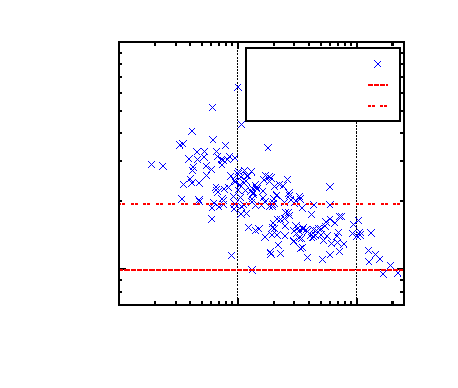
\includegraphics{medelsteg_lp}}%
    \gplfronttext
  \end{picture}%
\endgroup
}
\caption{}
\label{fig:storleksberoende}
\end{figure}





\section{Undersökning av olika typer av MSD}

För att avgöra hur väl approximationen för partikelrörelsen som en brownsk rörelse gäller kan man jämföra om vissa förutsägelser från teorin kring brownsk rörelse stämmer överens med vad som kan observeras från uppmätt data. Bland annat räknades det fram i avsnitt~\ref{sec:brown} att mean square displacement (MSD) för en sådan partikel skulle öka linjärt med tiden, se \eqref{eq:MSD_brown}.

Vidare finns det minst två sätt att beräkna partiklarnas MSD. För stationära processer, det vill säga processer som inte explicit beror på när i tiden de inleds, kan man skapa ett medelvärde mellan alla möjliga mätpunkter separerade med givet tidsintervall $\Delta{t}$ enligt
\begin{equation} \label{eq:MSD_S}
    S(\Delta t)= \frac{1}{N}\sum^N_{i=1}\frac{1}{m}\sum^m_{j=1}(x_i(t_j+\Delta t)-x_i(t_j))^2
\end{equation} 
där $N$ är antalet partiklar och $m$ antalet möjliga tidsintervall av längd $\Delta t$.
Genom att jämföra resultatet från denna typ av beräkning med att istället bara ta medelvärdet mellan alla partiklars kvadrerade radiella avvikelse från startpunkten vid given tid från start, det vill säga
\begin{equation} \label{eq:MSD_s}%Byta plats?
    s(\Delta t)= \frac{1}{N}\sum^N_{i=1}(x_i(\Delta t)-x_i(0))^2,
\end{equation} 
kan man avgöra om processen är stationär då dessa därmed borde ge samma resultat. 

En annan skillnad som kan uppstå när man beräknar MSD med \eqref{eq:MSD_S} respektive \eqref{eq:MSD_s} är att i en praktisk tillämpning, med begränsad datamängd, så kan $S(\Delta{t})$ bli betydligt jämnare än $s(\Delta{t})$. Detta på grund av att \eqref{eq:MSD_S} innehåller betydligt fler termer i varje medelvärde. 

\subsubsection{Databehandling}
Den studerade datan består av ett hundratal partiklar i respektive fas med, alla av olika storlek. Men då olika stora partiklar 

\todo[inline]{Utveckling pågår}

\subsection{Resultat -- MSD skiljer sig mellan de olika faserna}

För att undersöka om partikelrörelsen utgör en stationär process beräknas den stationära och icke-stationära MSD:n för partiklarna enligt ekvation \eqref{eq:MSD_S} och \eqref{eq:MSD_s}. Ett potenssamband har anpassats till resultaten i de båda beräkningarna och visas i figur \ref{fig:MSD}. 
Ingen väsentlig skillnad i exponenten kan uttydas från anpassningen mellan de båda MSD typerna, vilket tyder på att processen är stationär. Modellen tordes därför inom detta område beskrivas bättre av en stationär fBm snarare än en icke-stationär CTRW.

Jämförs exponenterna i potensanpassningen mellan energydepleted och logphase-cellerna, (a) respektive (b) i figur \ref{fig:MSD}, finns en markant skillnad. Exponenten för energydepleted cellerna är \todo{Samma antal värdesiffror i figurerna?} 0,65 mot logphase-cellernas 0,80. Båda processeran skiljer sig därmed från klassisk brownk rörelse där den förväntade exponenten är 1 \todo{Källa eller referens}\cite{}. Båda processerna är därmed exempel på subdiffusion, karakteriserat av att partikelns MSD beror av tiden via ett potenssamband med exponent mindre än 1 men större än 0. Då MSD:n ger en hint om hur snabbt partiklarna sprids verkar partiklarna i cellerna i dvala diffundera långsammare än partiklarna i de aktiva cellerna. De undersökta cellernas metabola tillstånd verkar alltså påverka diffusionen i cytoplasman vilket bekräftar resultat från tidigare studier~\cite{Parry_etal2014}. Dessa studier har, liksom här, utförts på celler utan motorprotein. Detta utesluter förklaringsmodellen där de utpekas som största bidragsfaktor som möjlig förklaring det det observerade fenomenet. 

Den icke-stationära MSD är som förväntat mer brusig än den stationära då färre medelvärden tas men samtidigt är linjen tillräckligt tydlig för att anpassningen ska kunna göras med liten felgräns.

\begin{figure}\centerline{
\subfigure[][]{
\resizebox{0.5\textwidth}{!}{% GNUPLOT: LaTeX picture with Postscript
\begingroup
  \makeatletter
  \providecommand\color[2][]{%
    \GenericError{(gnuplot) \space\space\space\@spaces}{%
      Package color not loaded in conjunction with
      terminal option `colourtext'%
    }{See the gnuplot documentation for explanation.%
    }{Either use 'blacktext' in gnuplot or load the package
      color.sty in LaTeX.}%
    \renewcommand\color[2][]{}%
  }%
  \providecommand\includegraphics[2][]{%
    \GenericError{(gnuplot) \space\space\space\@spaces}{%
      Package graphicx or graphics not loaded%
    }{See the gnuplot documentation for explanation.%
    }{The gnuplot epslatex terminal needs graphicx.sty or graphics.sty.}%
    \renewcommand\includegraphics[2][]{}%
  }%
  \providecommand\rotatebox[2]{#2}%
  \@ifundefined{ifGPcolor}{%
    \newif\ifGPcolor
    \GPcolorfalse
  }{}%
  \@ifundefined{ifGPblacktext}{%
    \newif\ifGPblacktext
    \GPblacktexttrue
  }{}%
  % define a \g@addto@macro without @ in the name:
  \let\gplgaddtomacro\g@addto@macro
  % define empty templates for all commands taking text:
  \gdef\gplbacktext{}%
  \gdef\gplfronttext{}%
  \makeatother
  \ifGPblacktext
    % no textcolor at all
    \def\colorrgb#1{}%
    \def\colorgray#1{}%
  \else
    % gray or color?
    \ifGPcolor
      \def\colorrgb#1{\color[rgb]{#1}}%
      \def\colorgray#1{\color[gray]{#1}}%
      \expandafter\def\csname LTw\endcsname{\color{white}}%
      \expandafter\def\csname LTb\endcsname{\color{black}}%
      \expandafter\def\csname LTa\endcsname{\color{black}}%
      \expandafter\def\csname LT0\endcsname{\color[rgb]{1,0,0}}%
      \expandafter\def\csname LT1\endcsname{\color[rgb]{0,1,0}}%
      \expandafter\def\csname LT2\endcsname{\color[rgb]{0,0,1}}%
      \expandafter\def\csname LT3\endcsname{\color[rgb]{1,0,1}}%
      \expandafter\def\csname LT4\endcsname{\color[rgb]{0,1,1}}%
      \expandafter\def\csname LT5\endcsname{\color[rgb]{1,1,0}}%
      \expandafter\def\csname LT6\endcsname{\color[rgb]{0,0,0}}%
      \expandafter\def\csname LT7\endcsname{\color[rgb]{1,0.3,0}}%
      \expandafter\def\csname LT8\endcsname{\color[rgb]{0.5,0.5,0.5}}%
    \else
      % gray
      \def\colorrgb#1{\color{black}}%
      \def\colorgray#1{\color[gray]{#1}}%
      \expandafter\def\csname LTw\endcsname{\color{white}}%
      \expandafter\def\csname LTb\endcsname{\color{black}}%
      \expandafter\def\csname LTa\endcsname{\color{black}}%
      \expandafter\def\csname LT0\endcsname{\color{black}}%
      \expandafter\def\csname LT1\endcsname{\color{black}}%
      \expandafter\def\csname LT2\endcsname{\color{black}}%
      \expandafter\def\csname LT3\endcsname{\color{black}}%
      \expandafter\def\csname LT4\endcsname{\color{black}}%
      \expandafter\def\csname LT5\endcsname{\color{black}}%
      \expandafter\def\csname LT6\endcsname{\color{black}}%
      \expandafter\def\csname LT7\endcsname{\color{black}}%
      \expandafter\def\csname LT8\endcsname{\color{black}}%
    \fi
  \fi
  \setlength{\unitlength}{0.0500bp}%
  \begin{picture}(4250.00,4534.00)%
    \gplgaddtomacro\gplbacktext{%
      \csname LTb\endcsname%
      \put(860,640){\makebox(0,0)[r]{\strut{}$10^{-9}$}}%
      \csname LTb\endcsname%
      \put(860,2228){\makebox(0,0)[r]{\strut{}$10^{-8}$}}%
      \csname LTb\endcsname%
      \put(860,3815){\makebox(0,0)[r]{\strut{}$10^{-7}$}}%
      \csname LTb\endcsname%
      \put(980,440){\makebox(0,0){\strut{} 0,01}}%
      \csname LTb\endcsname%
      \put(1950,440){\makebox(0,0){\strut{} 0,1}}%
      \csname LTb\endcsname%
      \put(2919,440){\makebox(0,0){\strut{} 1}}%
      \csname LTb\endcsname%
      \put(3889,440){\makebox(0,0){\strut{} 10}}%
      \put(160,2466){\rotatebox{-270}{\makebox(0,0){\strut{}$1-\text{CDF}$}}}%
      \put(2434,140){\makebox(0,0){\strut{}$\Delta{t}$ /[s]}}%
    }%
    \gplgaddtomacro\gplfronttext{%
      \csname LTb\endcsname%
      \put(3020,4080){\makebox(0,0)[r]{\strut{}\footnotesize $S(\Delta{t})$ energydepleted}}%
      \csname LTb\endcsname%
      \put(3020,3880){\makebox(0,0)[r]{\strut{}\footnotesize $s(\Delta{t})$ energydepleted}}%
      \csname LTb\endcsname%
      \put(3020,3680){\makebox(0,0)[r]{\strut{}\footnotesize Anpassning $\propto(\Delta{t})^{0,65}$}}%
    }%
    \gplbacktext
    \put(0,0){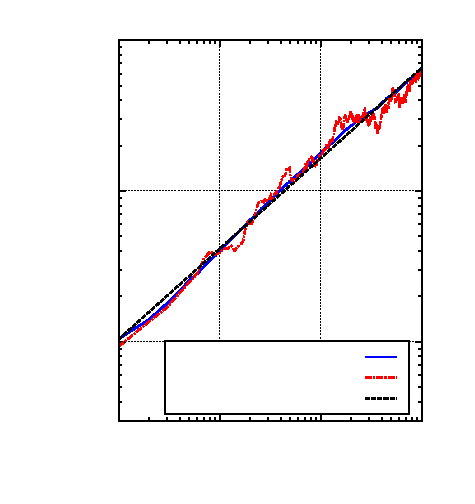
\includegraphics{MSD_ed}}%
    \gplfronttext
  \end{picture}%
\endgroup
}
}
\subfigure[][]{
\resizebox{0.5\textwidth}{!}{% GNUPLOT: LaTeX picture with Postscript
\begingroup
  \makeatletter
  \providecommand\color[2][]{%
    \GenericError{(gnuplot) \space\space\space\@spaces}{%
      Package color not loaded in conjunction with
      terminal option `colourtext'%
    }{See the gnuplot documentation for explanation.%
    }{Either use 'blacktext' in gnuplot or load the package
      color.sty in LaTeX.}%
    \renewcommand\color[2][]{}%
  }%
  \providecommand\includegraphics[2][]{%
    \GenericError{(gnuplot) \space\space\space\@spaces}{%
      Package graphicx or graphics not loaded%
    }{See the gnuplot documentation for explanation.%
    }{The gnuplot epslatex terminal needs graphicx.sty or graphics.sty.}%
    \renewcommand\includegraphics[2][]{}%
  }%
  \providecommand\rotatebox[2]{#2}%
  \@ifundefined{ifGPcolor}{%
    \newif\ifGPcolor
    \GPcolortrue
  }{}%
  \@ifundefined{ifGPblacktext}{%
    \newif\ifGPblacktext
    \GPblacktexttrue
  }{}%
  % define a \g@addto@macro without @ in the name:
  \let\gplgaddtomacro\g@addto@macro
  % define empty templates for all commands taking text:
  \gdef\gplbacktext{}%
  \gdef\gplfronttext{}%
  \makeatother
  \ifGPblacktext
    % no textcolor at all
    \def\colorrgb#1{}%
    \def\colorgray#1{}%
  \else
    % gray or color?
    \ifGPcolor
      \def\colorrgb#1{\color[rgb]{#1}}%
      \def\colorgray#1{\color[gray]{#1}}%
      \expandafter\def\csname LTw\endcsname{\color{white}}%
      \expandafter\def\csname LTb\endcsname{\color{black}}%
      \expandafter\def\csname LTa\endcsname{\color{black}}%
      \expandafter\def\csname LT0\endcsname{\color[rgb]{1,0,0}}%
      \expandafter\def\csname LT1\endcsname{\color[rgb]{0,1,0}}%
      \expandafter\def\csname LT2\endcsname{\color[rgb]{0,0,1}}%
      \expandafter\def\csname LT3\endcsname{\color[rgb]{1,0,1}}%
      \expandafter\def\csname LT4\endcsname{\color[rgb]{0,1,1}}%
      \expandafter\def\csname LT5\endcsname{\color[rgb]{1,1,0}}%
      \expandafter\def\csname LT6\endcsname{\color[rgb]{0,0,0}}%
      \expandafter\def\csname LT7\endcsname{\color[rgb]{1,0.3,0}}%
      \expandafter\def\csname LT8\endcsname{\color[rgb]{0.5,0.5,0.5}}%
    \else
      % gray
      \def\colorrgb#1{\color{black}}%
      \def\colorgray#1{\color[gray]{#1}}%
      \expandafter\def\csname LTw\endcsname{\color{white}}%
      \expandafter\def\csname LTb\endcsname{\color{black}}%
      \expandafter\def\csname LTa\endcsname{\color{black}}%
      \expandafter\def\csname LT0\endcsname{\color{black}}%
      \expandafter\def\csname LT1\endcsname{\color{black}}%
      \expandafter\def\csname LT2\endcsname{\color{black}}%
      \expandafter\def\csname LT3\endcsname{\color{black}}%
      \expandafter\def\csname LT4\endcsname{\color{black}}%
      \expandafter\def\csname LT5\endcsname{\color{black}}%
      \expandafter\def\csname LT6\endcsname{\color{black}}%
      \expandafter\def\csname LT7\endcsname{\color{black}}%
      \expandafter\def\csname LT8\endcsname{\color{black}}%
    \fi
  \fi
  \setlength{\unitlength}{0.0500bp}%
  \begin{picture}(4250.00,4534.00)%
    \gplgaddtomacro\gplbacktext{%
      \csname LTb\endcsname%
      \put(860,1397){\makebox(0,0)[r]{\strut{}$10^{-1}$}}%
      \csname LTb\endcsname%
      \put(860,2845){\makebox(0,0)[r]{\strut{}$10^{0}$}}%
      \csname LTb\endcsname%
      \put(860,4293){\makebox(0,0)[r]{\strut{}$10^{1}$}}%
      \csname LTb\endcsname%
      \put(980,440){\makebox(0,0){\strut{} 0,01}}%
      \csname LTb\endcsname%
      \put(1950,440){\makebox(0,0){\strut{} 0,1}}%
      \csname LTb\endcsname%
      \put(2919,440){\makebox(0,0){\strut{} 1}}%
      \csname LTb\endcsname%
      \put(3889,440){\makebox(0,0){\strut{} 10}}%
      \put(160,2466){\rotatebox{-270}{\makebox(0,0){\strut{}MSD $/\left[\text{godt. längdenhet}^2\right]$}}}%
      \put(2434,140){\makebox(0,0){\strut{}$\Delta{t}$ /[s]}}%
    }%
    \gplgaddtomacro\gplfronttext{%
      \csname LTb\endcsname%
      \put(3226,1253){\makebox(0,0)[r]{\strut{}\footnotesize $S(\Delta{t})$, log-fas}}%
      \csname LTb\endcsname%
      \put(3226,1053){\makebox(0,0)[r]{\strut{}\footnotesize $s(\Delta{t})$, log-fas}}%
      \csname LTb\endcsname%
      \put(3226,853){\makebox(0,0)[r]{\strut{}\footnotesize Anpassning $\propto(\Delta{t})^{0,8}$}}%
    }%
    \gplbacktext
    \put(0,0){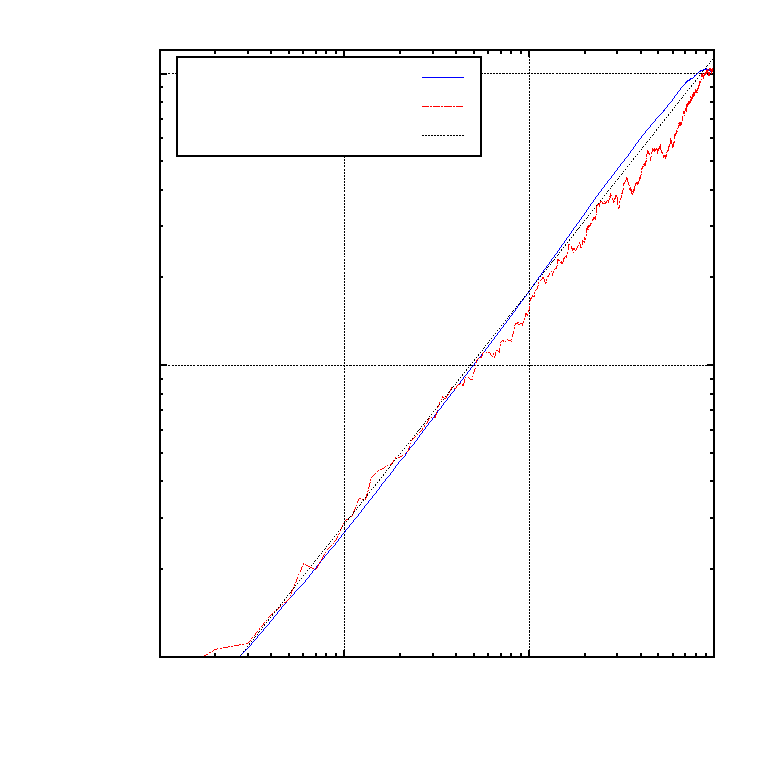
\includegraphics{MSD_lp}}%
    \gplfronttext
  \end{picture}%
\endgroup
}
}}
\caption{Log-logplott av de olika sorternas MSD, beräknade enligt \eqref{eq:MSD_S} respektive \eqref{eq:MSD_s}, för de olika cellfaserna, dvala (a) och aktiv (b). På grund av normeringen som användes kommer $S(\Delta{t})$ och  $s(\Delta{t})$ att ha samma värde i $\Delta{t}=\unit[10]{s}$. Detta är dock av liten betydelse eftersom det intressanta att undersöka är exponenten på $\Delta{t}$ (lutningen i dessa grafer). I de olika cellfaserna syns att lutningarna i diagrammen är samma inom varje fas, men skiljger sig åt mellan (a) och (b). Detta tyder på ett stationärt beteende, men att det ändå finns en tydlig skilnad mellan aktiva celler och de i dvala. Notera också att $S$ är jämnare än $s$, vilket bara beror på att $S$ innehåller fler termer som medelvärderats. }
\label{fig:MSD}
\end{figure}


\section{Spektraltäthet och brushantering}
Ett annat verktyg för att undersöka partilarnas rörelser är att titta på vad för spektraltäthet partiklarnas position har. Spektraltätheten erhålls genom att ta Fouriertransformen av partikelns position som funktion av tid. På så sätt erhålls ett mått på hur mycket av varje frekvens som finns. Detta kan vara användbart på flera olika sätt; bland annat ger det ett annat sätt att \todo{Jag vet fortfarande inte hur man gör här}ta fram hur MSD:n beter sig, men spektraltätheten kan också användas för att 

Om man 
\begin{equation}
\hat{x} = x + \sigma\eta
\end{equation}


\todo[inline]{Mer kommer sen.}

Ett annat sätt att upptäcka bruset i en mätning är att titta på...


\subsection{Resultat -- }


\section{Anisotropi i partikelrörelsen}
\todo[inline]{Gör om simuleringarna med riktiga kovarianser! (Som ekvationerna nedan är skrivna nu.)}
Om man misstänker att cellens inre struktur påverkar partikelrörelserna skulle eventuell anisotropi kunna ge ett bidrag till dessa. Alltså ifall det finns föredragna riktningar för partikeln att röra sig i. Ett sätt att undersöka detta är genom att betrakta koordinaternas \todo{Anpassa till kap. 2!}kovarianstensor som är en tensor med de olika koordinaternas statistiska andramoment:
\begin{equation}
C_{ij} = \frac{1}{N} \sum_{n=1}^{N} 
\left(r_i^{(n)}r_j^{(n)} -\bar{r}_i\bar{r}_j \right),
\end{equation}
där $r_i^{(n)}$ är den $i$:te koordinaten ($x$ eller $y$) i den $n$:te datapunkten och $\bar{r}_i$ är den $i$:te koordinatens medelvärde. På matrisform kan $C$ skrivas som
\begin{equation}\label{eq:C_matris}
C=
\begin{bmatrix} 
\ev{x^2}-\ev{x}^2 & \ev{xy}-\ev{x}\ev{y}\\
\ev{yx}-\ev{x}\ev{y} & \ev{y^2}-\ev{y}^2
\end{bmatrix}.
\end{equation}

Notera hur snarlik $C$ är med tröghetstensorn för en kropps olika tröghetsmoment som uppkommer i mekaniken. Och precis som i mekaniken kan man hitta två principalaxlar genom att ta fram dess egenvektorer och diagonalisera tensorn. I mekaniken svarar principalaxlarna mot de riktningar av rörelsemängdsmoment som är oberoende av rotation längs andra axlar. I de här statistiska sammanhangen finns det en liknande tolkning nämligen att principalaxlarna svarar mot de riktningar i cellen där rörelserna är oberoende av varandra. Egenvärdena i dessa två riktningarna svarar mot variansen i den oberoende koordinaten längs med den riktningen.

För att ur kovarianstensorn få ut ett mått på hur isotropt partikeln rör sig kan man undersöka asymmetrimåttet~\cite{Rudnick_Asphericity1986}
\begin{equation}\label{eq:asph.}
    A_d=\frac{\sum_{j}\sum_{i<j} 
\ev{(\lambda_i-\lambda_j)^2} }{
(d-1) \ev{(\sum_j \lambda_j)^2}}
\end{equation}
i $d$ dimensioner, kallat \emph{asfärisitet}. Egenvärdena själva svarar som sagt mot variansen i de olika riktningarna, vilket motsvarar hur mycket partikeln har rört sig i respektive rikting. Hade positionerna varit helt isotropt fördelade så hade alltså $A=0$, om partikeln bara hade rört sig längs en linje blir istället $A=1$.
I två dimensioner förenklas \eqref{eq:asph.} till 
\begin{equation}\label{eq:asph._2D}
    A=\frac{\ev{(\lambda_1 - \lambda_2)^2}}{\ev{(\lambda_1 + \lambda_2)^2}}.
\end{equation}

\subsubsection{Tillämpning av asfärisiteten}
Man kan enkelt visa att egenvärdena till kovarianstensorn i \eqref{eq:C_matris} uppfyller~\cite{Hong_asymmetri1998}
\begin{equation}
\begin{aligned}
    \lambda_1+\lambda_2 &= \ev{x^2}+\ev{y^2} \\
    \abs{\lambda_1-\lambda_2} &= 
        \sqrt{\left(\ev{x^2}-\ev{y^2}\right)^2 + 4\ev{xy}^2}.
\end{aligned}
\end{equation}
För en given fördelningsfunktion med ändliga moment blir det därmed nu möjligt att beräkna denna kvot teoretiskt.

För en obegränsad Wienerprocess i $d$ dimensioner fås 
\begin{equation} \label{eq:Asphericity_Brownian}
    A_d^\text{(Wierner)}=\frac{2(d+2)}{5d+4}.
\end{equation}
För två dimensioner fås $A_2^\text{(Wierner)}=\nicefrac{4}{7}$. Detta innebär att även långvariga slumpvandringar i snitt kommer att uppvisa viss anisotropi.

För fBm fås en approximativ formel i två dimensioner i gränsen där antalet mätpunkter blir mycket stort ~\cite{Hong_asymmetri1998}
\begin{equation} \label{eq:A_fBm}
A=2-
\frac{\frac{1}{2(H+1)^2}}{\frac{1}{2(H+1)^2}+\frac{2H+1}{4(4H+1)}-\frac{1}{4H+3}-\frac{\Gamma^2(2H+2)}{\Gamma(4H+4)}},
\end{equation}
där $H$ är Hurst parametern som karakteriserar rörelsen och $\Gamma$ gamma-funktionen. För $H=\nicefrac{1}{2}$ fås en vanlig brownsk rörelse med motsvarande  asymmetrimått $A=\nicefrac{4}{7}$ vilket stämmer överens med ekvation \eqref{eq:Asphericity_Brownian} för $d=2$. Samma värde fås även approximativt för CTRW-modellen \cite{Ernst_ACTRW2012} då denna rörelse vid varje tidsögonblick ser ut som brownsk rörelse. \todo{Vad menas här? Kolla upp}.

%Även http://iopscience.iop.org/article/10.1088/0305-4470/19/4/004/pdf



 
\subsection{Simulering och numerisk beräkning av asymmetrimått} %Något om egenvärdes kvoter i titel
Istället för att bara direkt beräkna $A$ enligt \eqref{eq:asph._2D} för den undersökta datan och några olika modeller kan man också studera fördelningen av måttet 
\begin{equation}
\varLambda = 
\frac{(\lambda_1 - \lambda_2)^2}{(\lambda_1 + \lambda_2)^2}.
\end{equation}
Här ska det dock påpekas att det inte går att få $A$ från  $\ev{\varLambda}$ eftersom \eqref{eq:asph._2D} består av ett väntevärde i både täljare och nämnare. Eftersom $\varLambda$ alltså skiljer sig så från $A$ går det heller inte lika enkelt att göra teoretiska beräkningar, vilket gör att fördelningen av $\varLambda$ får undersökas med Monte Carlo-simuleringar.


%Eftersom en mätning bara kan bestå av ett ändligt antal datapunkter kan även en äkta, isotrop brownsk rörelse ge upphov till $\varLambda>1$. Vidare är \emph{kvoten} mellan egenvärden inte linjär, vilket gör en teoretisk analys av fördelningarna mycket svår. För att ändå kunna säga något om den riktiga datan kan man ganska enkelt ta fram en fördelning för $\varLambda$ för några olika modeller genom simulering. 

De modeller som testats är en vanlig Wienerprocess, en Wienerprocess med ett ''mätbrus'' pålagt och en Ornstein-Uhlenbeck-process. Från dessa processer samt från datan över partikelrörelsen erhölls olika fördelningar av $\varLambda$. 


Wienerprocessen simulerade fram partikelns position i varje ny tidpunkt genom att gå ett normalfördelat steg från positionen i den förra tidpunkten. Detta kan skrivas som
\begin{equation}\label{eq:sim_wiener}
x_{i+1} = x_i + \delta 
\qcomma  \delta \sim N(0, \sigma)
\end{equation}
och där $x_1=0$. Sedan gör man samma sak för $y$. Eftersom $\varLambda$ ger ett mått på hur mycket partikeln \emph{föredrar en viss riktning}, finner man att värdet på $\sigma$ inte påverkar fördelningen -- så länge $\sigma$ är samma för både $x$ och $y$. Detta blir uppenbart när man tänker på att \eqref{eq:sim_wiener} kan skrivas som 
\begin{equation}
x_{i+1} =\sigma\,\hat{x}_{i+i} = \sigma\,\left( \hat{x}_i + \hat{\delta} \right) 
\qcomma  \hat{\delta} \sim N(0, 1).
\end{equation}
Alltså att $\sigma$ bara är en multiplikativ konstant framför positionen.

För att istället simulera en Wienerprocess med mätbrus användes \eqref{eq:sim_wiener} för att först simulera själva Wienerprocessen för att sedan \emph{efteråt} addera en slumpad brusterm $\eta \sim N(0, \sigma')$ till varje $x_i$. Den väsentliga skillnaden mot en ren Wienerprocess är att mätbruset $\eta$ inte påverkar nästkommande position. Till skillnad från den rena Wienerprocessen så kommer värdena på $\sigma$ och $\sigma'$ att påverka $\varLambda$, men enligt samma argument som ovan kommer bara kvoten $\nicefrac{\sigma'}{\sigma}$ vara det som påverkar. Detta gör att simuleringarna med mätbrus går att genomföra med olika värden på parametern $\nicefrac{\sigma'}{\sigma}$ för att få olika fördelningar av $\varLambda$. 

Ornstein-Uhlenbeck-processen i \eqref{eq:SDE_o-u} simulerades genom att använda derivatan för tidsutveckling och genom att sätta $\bar{x}=0$. Man får då
\begin{equation}
x_{i+1} = x_i + \Delta{t}\,\pd_{t}x  = (1-k) x_i +  \delta 
\qcomma  \delta \sim N(0, \sigma),
\end{equation}
där $x_1=0$. Notera här att den styrande parametern i simuleringarna är $k=\gamma\Delta{t}$, samt att $\sigma$ på samma sätt som för den rena Wienerprocessen kan väljas godtyckligt utan att påverka $\varLambda$. 

Eftersom resultatet för asymmetrimåttet i ekvation \eqref{eq:A_fBm} gäller för riktigt långa mätningar medan den data som analyseras i detta arbete är ganska begränsad kan man försöka simulera fram sannolikheter istället. Genom att simulera många mätserier för samma antal steg och antal partiklar som i datan kan man bedöma sannolikheten att det framräknade asymmetrimåttet till exempel skulle ha kommit från en ren klassisk brownsk rörelse. 

\subsection{Resultat -- partikelrörelsen är mer isotrop än brownsk rörelse}
En anledning till att kolla om en tydlig asymmetri kan uttydas ur datan över partiklarnas rörelse är att bedöma hurvida man istället för de givna x- och y-koordinaterna bör gå över till tangential- och normalkoordinater. Eftersom ingen sådan uttalad assymetri verkar finnas borde koordinatsystemet lämnas som det är.

Genom att spela upp datan över partikelpositionerna som en film blir det tydligt att vissa partiklar stöter på större strukturer i cytoplasman som de inte kan rubba ur vägen utan måste ta sig runt. För dessa partiklar ter sig cytoplasman alltså inte helt isotrop på större tidsskalor. \todo{Vad kan man säga mer här?}

%Mer isotropt än vid brownsk rörelse. Påverkas kanske av cellens inre utformning och hålls på plats

%\begin{figure}\centering
%% GNUPLOT: LaTeX picture with Postscript
\begingroup
  \makeatletter
  \providecommand\color[2][]{%
    \GenericError{(gnuplot) \space\space\space\@spaces}{%
      Package color not loaded in conjunction with
      terminal option `colourtext'%
    }{See the gnuplot documentation for explanation.%
    }{Either use 'blacktext' in gnuplot or load the package
      color.sty in LaTeX.}%
    \renewcommand\color[2][]{}%
  }%
  \providecommand\includegraphics[2][]{%
    \GenericError{(gnuplot) \space\space\space\@spaces}{%
      Package graphicx or graphics not loaded%
    }{See the gnuplot documentation for explanation.%
    }{The gnuplot epslatex terminal needs graphicx.sty or graphics.sty.}%
    \renewcommand\includegraphics[2][]{}%
  }%
  \providecommand\rotatebox[2]{#2}%
  \@ifundefined{ifGPcolor}{%
    \newif\ifGPcolor
    \GPcolorfalse
  }{}%
  \@ifundefined{ifGPblacktext}{%
    \newif\ifGPblacktext
    \GPblacktexttrue
  }{}%
  % define a \g@addto@macro without @ in the name:
  \let\gplgaddtomacro\g@addto@macro
  % define empty templates for all commands taking text:
  \gdef\gplbacktext{}%
  \gdef\gplfronttext{}%
  \makeatother
  \ifGPblacktext
    % no textcolor at all
    \def\colorrgb#1{}%
    \def\colorgray#1{}%
  \else
    % gray or color?
    \ifGPcolor
      \def\colorrgb#1{\color[rgb]{#1}}%
      \def\colorgray#1{\color[gray]{#1}}%
      \expandafter\def\csname LTw\endcsname{\color{white}}%
      \expandafter\def\csname LTb\endcsname{\color{black}}%
      \expandafter\def\csname LTa\endcsname{\color{black}}%
      \expandafter\def\csname LT0\endcsname{\color[rgb]{1,0,0}}%
      \expandafter\def\csname LT1\endcsname{\color[rgb]{0,1,0}}%
      \expandafter\def\csname LT2\endcsname{\color[rgb]{0,0,1}}%
      \expandafter\def\csname LT3\endcsname{\color[rgb]{1,0,1}}%
      \expandafter\def\csname LT4\endcsname{\color[rgb]{0,1,1}}%
      \expandafter\def\csname LT5\endcsname{\color[rgb]{1,1,0}}%
      \expandafter\def\csname LT6\endcsname{\color[rgb]{0,0,0}}%
      \expandafter\def\csname LT7\endcsname{\color[rgb]{1,0.3,0}}%
      \expandafter\def\csname LT8\endcsname{\color[rgb]{0.5,0.5,0.5}}%
    \else
      % gray
      \def\colorrgb#1{\color{black}}%
      \def\colorgray#1{\color[gray]{#1}}%
      \expandafter\def\csname LTw\endcsname{\color{white}}%
      \expandafter\def\csname LTb\endcsname{\color{black}}%
      \expandafter\def\csname LTa\endcsname{\color{black}}%
      \expandafter\def\csname LT0\endcsname{\color{black}}%
      \expandafter\def\csname LT1\endcsname{\color{black}}%
      \expandafter\def\csname LT2\endcsname{\color{black}}%
      \expandafter\def\csname LT3\endcsname{\color{black}}%
      \expandafter\def\csname LT4\endcsname{\color{black}}%
      \expandafter\def\csname LT5\endcsname{\color{black}}%
      \expandafter\def\csname LT6\endcsname{\color{black}}%
      \expandafter\def\csname LT7\endcsname{\color{black}}%
      \expandafter\def\csname LT8\endcsname{\color{black}}%
    \fi
  \fi
  \setlength{\unitlength}{0.0500bp}%
  \begin{picture}(6802.00,4534.00)%
    \gplgaddtomacro\gplbacktext{%
      \csname LTb\endcsname%
      \put(946,704){\makebox(0,0)[r]{\strut{}$10^{-2}$}}%
      \csname LTb\endcsname%
      \put(946,2487){\makebox(0,0)[r]{\strut{}$10^{-1}$}}%
      \csname LTb\endcsname%
      \put(946,4269){\makebox(0,0)[r]{\strut{}$10^{0}$}}%
      \csname LTb\endcsname%
      \put(1078,484){\makebox(0,0){\strut{} 1}}%
      \csname LTb\endcsname%
      \put(2852,484){\makebox(0,0){\strut{} 10}}%
      \csname LTb\endcsname%
      \put(4626,484){\makebox(0,0){\strut{} 100}}%
      \put(176,2486){\rotatebox{-270}{\makebox(0,0){\strut{}MSD $/\left[\text{godt. längdenhet}^2\right]$}}}%
      \put(2852,154){\makebox(0,0){\strut{}$\varLambda$}}%
    }%
    \gplgaddtomacro\gplfronttext{%
      \csname LTb\endcsname%
      \put(6078,4159){\makebox(0,0)[r]{\strut{}kvot}}%
      \csname LTb\endcsname%
      \put(6078,3939){\makebox(0,0)[r]{\strut{}brus 14}}%
      \csname LTb\endcsname%
      \put(6078,3719){\makebox(0,0)[r]{\strut{}brus 9}}%
      \csname LTb\endcsname%
      \put(6078,3499){\makebox(0,0)[r]{\strut{}dvala}}%
      \csname LTb\endcsname%
      \put(6078,3279){\makebox(0,0)[r]{\strut{}aktiv}}%
      \csname LTb\endcsname%
      \put(6078,3059){\makebox(0,0)[r]{\strut{}spring 2,6\,s}}%
      \csname LTb\endcsname%
      \put(6078,2839){\makebox(0,0)[r]{\strut{}spring 6,0\,s}}%
    }%
    \gplbacktext
    \put(0,0){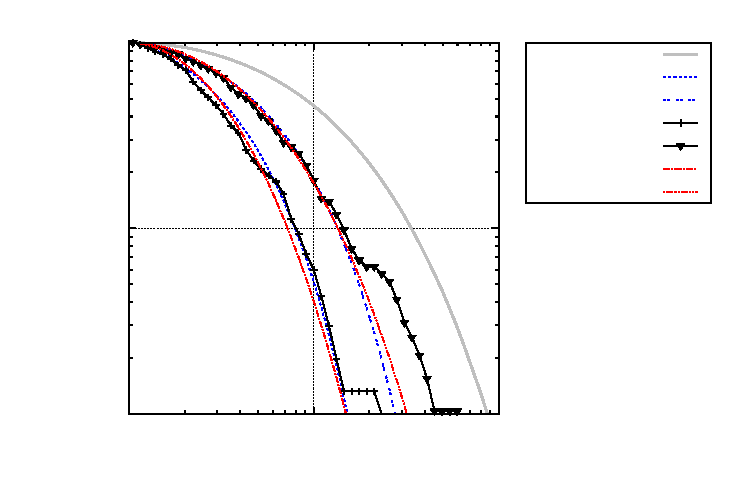
\includegraphics{isotropi_kvot}}%
    \gplfronttext
  \end{picture}%
\endgroup
 
%\caption{}
%\label{fig:fordelning_kvot}
%\end{figure}

\begin{figure}\centering
% GNUPLOT: LaTeX picture with Postscript
\begingroup
  \makeatletter
  \providecommand\color[2][]{%
    \GenericError{(gnuplot) \space\space\space\@spaces}{%
      Package color not loaded in conjunction with
      terminal option `colourtext'%
    }{See the gnuplot documentation for explanation.%
    }{Either use 'blacktext' in gnuplot or load the package
      color.sty in LaTeX.}%
    \renewcommand\color[2][]{}%
  }%
  \providecommand\includegraphics[2][]{%
    \GenericError{(gnuplot) \space\space\space\@spaces}{%
      Package graphicx or graphics not loaded%
    }{See the gnuplot documentation for explanation.%
    }{The gnuplot epslatex terminal needs graphicx.sty or graphics.sty.}%
    \renewcommand\includegraphics[2][]{}%
  }%
  \providecommand\rotatebox[2]{#2}%
  \@ifundefined{ifGPcolor}{%
    \newif\ifGPcolor
    \GPcolorfalse
  }{}%
  \@ifundefined{ifGPblacktext}{%
    \newif\ifGPblacktext
    \GPblacktexttrue
  }{}%
  % define a \g@addto@macro without @ in the name:
  \let\gplgaddtomacro\g@addto@macro
  % define empty templates for all commands taking text:
  \gdef\gplbacktext{}%
  \gdef\gplfronttext{}%
  \makeatother
  \ifGPblacktext
    % no textcolor at all
    \def\colorrgb#1{}%
    \def\colorgray#1{}%
  \else
    % gray or color?
    \ifGPcolor
      \def\colorrgb#1{\color[rgb]{#1}}%
      \def\colorgray#1{\color[gray]{#1}}%
      \expandafter\def\csname LTw\endcsname{\color{white}}%
      \expandafter\def\csname LTb\endcsname{\color{black}}%
      \expandafter\def\csname LTa\endcsname{\color{black}}%
      \expandafter\def\csname LT0\endcsname{\color[rgb]{1,0,0}}%
      \expandafter\def\csname LT1\endcsname{\color[rgb]{0,1,0}}%
      \expandafter\def\csname LT2\endcsname{\color[rgb]{0,0,1}}%
      \expandafter\def\csname LT3\endcsname{\color[rgb]{1,0,1}}%
      \expandafter\def\csname LT4\endcsname{\color[rgb]{0,1,1}}%
      \expandafter\def\csname LT5\endcsname{\color[rgb]{1,1,0}}%
      \expandafter\def\csname LT6\endcsname{\color[rgb]{0,0,0}}%
      \expandafter\def\csname LT7\endcsname{\color[rgb]{1,0.3,0}}%
      \expandafter\def\csname LT8\endcsname{\color[rgb]{0.5,0.5,0.5}}%
    \else
      % gray
      \def\colorrgb#1{\color{black}}%
      \def\colorgray#1{\color[gray]{#1}}%
      \expandafter\def\csname LTw\endcsname{\color{white}}%
      \expandafter\def\csname LTb\endcsname{\color{black}}%
      \expandafter\def\csname LTa\endcsname{\color{black}}%
      \expandafter\def\csname LT0\endcsname{\color{black}}%
      \expandafter\def\csname LT1\endcsname{\color{black}}%
      \expandafter\def\csname LT2\endcsname{\color{black}}%
      \expandafter\def\csname LT3\endcsname{\color{black}}%
      \expandafter\def\csname LT4\endcsname{\color{black}}%
      \expandafter\def\csname LT5\endcsname{\color{black}}%
      \expandafter\def\csname LT6\endcsname{\color{black}}%
      \expandafter\def\csname LT7\endcsname{\color{black}}%
      \expandafter\def\csname LT8\endcsname{\color{black}}%
    \fi
  \fi
  \setlength{\unitlength}{0.0500bp}%
  \begin{picture}(6802.00,4534.00)%
    \gplgaddtomacro\gplbacktext{%
      \csname LTb\endcsname%
      \put(814,704){\makebox(0,0)[r]{\strut{}$0$}}%
      \csname LTb\endcsname%
      \put(814,1417){\makebox(0,0)[r]{\strut{}$0,2$}}%
      \csname LTb\endcsname%
      \put(814,2130){\makebox(0,0)[r]{\strut{}$0,4$}}%
      \csname LTb\endcsname%
      \put(814,2843){\makebox(0,0)[r]{\strut{}$0,6$}}%
      \csname LTb\endcsname%
      \put(814,3556){\makebox(0,0)[r]{\strut{}$0,8$}}%
      \csname LTb\endcsname%
      \put(814,4269){\makebox(0,0)[r]{\strut{}$1$}}%
      \csname LTb\endcsname%
      \put(946,484){\makebox(0,0){\strut{} 0}}%
      \csname LTb\endcsname%
      \put(1682,484){\makebox(0,0){\strut{} 0,2}}%
      \csname LTb\endcsname%
      \put(2418,484){\makebox(0,0){\strut{} 0,4}}%
      \csname LTb\endcsname%
      \put(3154,484){\makebox(0,0){\strut{} 0,6}}%
      \csname LTb\endcsname%
      \put(3890,484){\makebox(0,0){\strut{} 0,8}}%
      \csname LTb\endcsname%
      \put(4626,484){\makebox(0,0){\strut{} 1}}%
      \put(176,2486){\rotatebox{-270}{\makebox(0,0){\strut{}MSD $/\left[\text{godt. längdenhet}^2\right]$}}}%
      \put(2786,154){\makebox(0,0){\strut{}$\varLambda$}}%
    }%
    \gplgaddtomacro\gplfronttext{%
      \csname LTb\endcsname%
      \put(6078,4159){\makebox(0,0)[r]{\strut{}kvot}}%
      \csname LTb\endcsname%
      \put(6078,3939){\makebox(0,0)[r]{\strut{}brus 14}}%
      \csname LTb\endcsname%
      \put(6078,3719){\makebox(0,0)[r]{\strut{}brus 9}}%
      \csname LTb\endcsname%
      \put(6078,3499){\makebox(0,0)[r]{\strut{}dvala}}%
      \csname LTb\endcsname%
      \put(6078,3279){\makebox(0,0)[r]{\strut{}aktiv}}%
      \csname LTb\endcsname%
      \put(6078,3059){\makebox(0,0)[r]{\strut{}spring 2,6\,s}}%
      \csname LTb\endcsname%
      \put(6078,2839){\makebox(0,0)[r]{\strut{}spring 6,0\,s}}%
    }%
    \gplbacktext
    \put(0,0){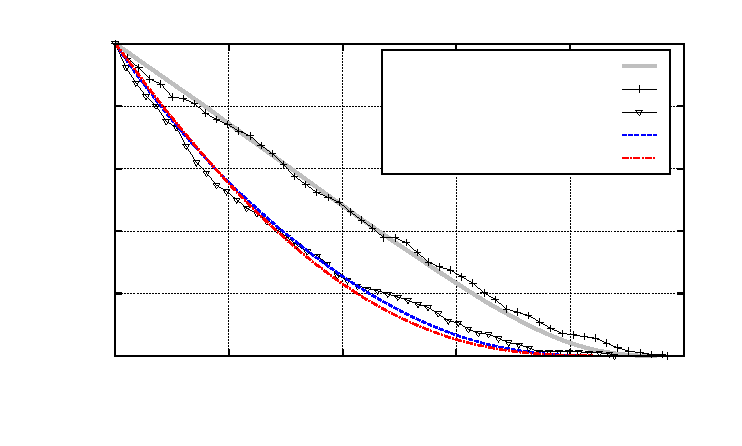
\includegraphics{isotropi_asymmetri}}%
    \gplfronttext
  \end{picture}%
\endgroup

\caption{}
\label{fig:asymmetri}
\end{figure}



\section{Diskussion}
\todo[inline]{Inga tomma rubriker}

\subsection{Ornstein-Uhlenbeck-modellen}
\todo[inline]{Varsågod att ändra så mycket ni vill.}


%Om sambandet mellan intensitet och partikelstorleken påverkar resultatet

%Byter man till normal- och tangential-koordinater bygger man in ett bias som påverkar resultaten till att det verkar finnas egenskaper som egentligen inte finns. 
%Av slumpskäl kommer vissa vägar att vara mer raka än andra medan andra får mer symmetriska banor.


%Bara en liten kodsnutt som behövs när man kompilerar lokalt
%%% Local Variables: 
%%% mode: latex
%%% TeX-master: "00main.tex"
%%% End: 